% siminos/blog/CLEflotsam
% $Author$ $Date$
%
% Predrag transfered to here from siminos/CLE/      Jun  5 2010
% Predrag created file siminos/CLE/flotsam.tex      Dec 20 2009

\chapter{CLE flotsam}

%    \PC{
%    remove PC\{\} and PCedit\{\}, \etc,
%    after you have accepted/edited them
%    }
This section contains material which has not been included in
publication
{\tt siminos/CLE/CLE.tex}.

{\bf PC 2010-06-07 moved this into example in ChaosBook.org}:
``
When one takes syzygies into account in rewriting the
dynamical system, singularities are introduced. [...]
''

{\bf ES 2009-12-21:}
In {\cLe} a secondary
bifurcation from \REQV{}{1} is expected, according to Krupa's
theorem\rf{Krupa90}, to result in \emph{relative periodic
orbits}.

{\bf ES 2009-12-21 rephrased:}
``To cite Fels and Olver\rf{FelsOlver98}:
moving frames where ``first introduced by Gaston Darboux
and brought to maturity by \'Elie Cartan.''
''

{\bf ES 2009-12-21 dropped:}
``
\SOn{2} acts regularly and freely on
$X^*=\Rls{5}\backslash\{x_1=x_2=y_1=y_2=0\}$ and thus we are
guaranteed to find the fundamental invariants by the method
of moving frames if we restrict attention to $X^*$.
''

A generic  $ \slicep $ can be brought to form $ \slicep  =
(0,1,y_1^{*},y_2^{*})$ by a rotation and rescaling. Then $\Lg
\cdot \slicep   = (1,0,y_2^{*},-y_1^{*})$, and
\beq
\frac{(\vel \cdot \Lg \cdot \slicep )}{(\ssp \cdot\slicep )_4} =
\frac{\vel_1 + \vel_3 y^{*}_2 -\vel_4 y^{*}_1}
     {x_2 + y_1 y^{*}_1 + y_2 y^{*}_2}
%\frac{\vel_1 x^{*}_2 -\vel_2 x^{*}_1 + \vel_3 y^{*}_2 -\vel_4 y^{*}_1}
%     {\vel_1 x^{*}_1 + \vel_2 x^{*}_2 + \vel_3 y^{*}_1 + \vel_4 y^{*}_2}
\,.
\label{PCsectSin1}
\eeq


 {\bf ES 2009-12-21 dropped (and PC agrees):}
``
We say that $\Group$ acts locally freely on \pS\ if for any
$\ssp\in\pS$ the isotropy subgroup $\stab{\ssp}$ is a
discrete subgroups of $\Group$. An r-dimensional compact Lie
group $\Group$ acts \emph{locally freely} on $\pS$ if and
only if it has $r-dimensional$ orbits\rf{FelsOlver99}. A
group $\Group$ acts freely on $\pS$ if all isotropy subgroups
are trivial: \stab{\ssp}=\{e\} for all $\ssp\in \Manif$. If
in addition for each point $\ssp\in \Manif$ there exists an
arbitrarily small neighborhood $U$ such that each orbit of
$\Group$ intersects $U$ in a pathwise connected subset, then
the group acts regularly.
''

{\bf ES 2009-12-21 dropped:}
``
A group $\Group$ acts semi-regularly on $\pS$ if all its
orbits have the same dimension. Therefore the group orbits of
a group that acts semi-regularly foliate $\pS$. A sufficient
condition for a semi-regular action is that for any
$\ssp\in\pS$ the isotropy subgroup $\stab{\ssp}$ is a
discrete subgroup of $\Group$. If a Lie group $\Group$ acts
semi-regularly on a manifold $\Manif$,

Note that locally free action implies semi-regular action.
''

{\bf ES 2010-01-22 dropped:}
``
In this section we present the {\mframes}, introduced by G. Darboux and
systematized by \'E. Cartan\rf{CartanMF}.
Fels and Olver\rf{FelsOlver98,FelsOlver99} reformulated the method so that a
moving frame is simply an equivariant mapping from the space on which a
group acts to the group parameter.  In refsect~{s:mfReqb} we will
exploit the geometric interpretation of moving frames for a more direct and
efficient approach to symmetry reduction. \refrefs{FelsOlver98,FelsOlver99}

A moving frame is a smooth
$\Group$-equivariant mapping $\rho$ from $\Manif$ to the
$\Group$, that is to the group parameters.

One distinguishes between left moving frames for which
the equivariance condition is $\rho(\LieEl x)=\LieEl\rho(x)\,,\
x\in\Manif\,,\ \LieEl\in\Group$ and right moving frames for
which the equivariance condition is $\rho(\LieEl
x)=\rho(x)\LieEl^{-1}\,,\ x\in\Manif\,,\ \LieEl\in\Group$.  As shown in \refref{FelsOlver99} a moving frame exists
in a neighborhood of a point $x\in\Manif$ if and only if
$\Group$ acts freely and regularly near x.

For the practical
construction of a moving frame for an $N-$dimensional Lie group
$\Group$ we will need to define a slice.
Therefore the existence of a moving frame depends on
group orbits having the same dimension.

re-insert?: To construct a moving frame, let $K\subset\Manif$ be a {\slice}. For $x\in \Manif$, let
$\LieEl=\rho(x)$ be the unique group element that maps $x$
to the {\slice}: $g x = \rho(x) x\, \in K$. Then
$\rho:\Manif\rightarrow \Group$ is a right moving frame\rf{FelsOlver98}.

A {\slice} $K$ can be defined by means of level sets of
functions $K_i(x)=c_i$, where $x\in V$ and $i=1,\ldots,r$. If
the $K_i(x)$ coincide with the local coordinates $x_i$ on the
manifold $V$, \ie~$K_i(x)=x_i$,
..

{\bf ES:}
Moved example from movingFrames.tex here, some bits should still be rescued.

In this section we illustrate symmetry reduction through
the use of invariants computed
with the moving frame method in the example of \cLe.
The $z$-axis is the \fixedsp\ of \SOn{2} acting by
\refeq{eq:SO2act} on \Rls{5}. Therefore we can define
a coordinate {\slice} on $\Rls{5}\backslash\{x_1=x_2=y_1=y_2=0\}$
by, for instance,
\beq%\label{eq:CLEsliceSO2}
x_1=0,\,x_2>0\,.
\eeq
We can now construct a moving frame for the action
\refeq{eq:SO2act} of $\SOn{2}$ as follows. We write out
explicitly the group transformations:
\begin{subequations}%\label{eq:CLEnorm}
\begin{align}
 	\overline{x}_1 &= x_1 \cos\theta - x_2 \sin\theta\cont
	\overline{x}_2 &= x_1 \sin\theta + x_2 \cos\theta\cont
	\overline{y}_1 &= y_1 \cos\theta - y_2 \sin\theta\cont
	\overline{y}_2 &= y_1 \sin\theta + y_2 \cos\theta\cont	
	\overline{z} &= z\,.
\end{align}
\end{subequations}
We set $\overline{x}_1=0$ and solve
\refeq{eq:CLEexplSO2a} for the group parameter to obtain the moving frame
\beq
	\theta=\tan^{-1}\frac{x_1}{x_2}
% 	\label{eq:CLEmf}
\eeq
which brings any point  back to the {\slice}.
Here it is important that
$\tan^{-1}$ distinguishes quadrants in the $(x_1,x_2)$ plane to ensure that the
transformation results in the correct geometric
interpretation, \ie\ to ensure $x_2>0$.
Substituting \refeq{eq:CLEmf} in the remaining equations \refeq{eq:CLEnorm} we
get the invariants
\beq
\begin{split}
	\overline{x}_2 &=  r_1 = \sqrt{x_1^2+x_2^2} \cont
	\overline{y}_1 &= {(x_2 y_1-x_1 y_2)}/{r_1}\cont
	\overline{y}_2 &= {(x_1 y_1+x_2 y_2)}/{r_1}\cont	
	\overline{z} &= z\,.
% 	\label{eq:invLaser}
\end{split}
\eeq
{\bf ES:} The solution $\theta = 2
    \tan^{-1}\frac{-x_2+\sqrt{x_1^2+x_2^2}}{x_1}$ was
    returned by Mathematica. If we use $\theta =
    \tan^{-1}\frac{x_2}{x_1}$ without taking care of the
    quadrant our results are multiplied by $sgn(x_2)$.


{\bf ES: I will need to rewrite the following}

In terms of projecting dynamics
on variables \refeq{eq:invLaser} (or applying the equivalent
procedure of rotating points back to the \slice) this means that
we need to take into account the direction along which
we approach zero and use the `angle
of descent' as the angle with which we rotate points back to the \slice, if such
points have exactly $x=0$.

Note that the invariants are not defined on
the subspace $U_S$ defined by $x_1=x_2=0$ even though the
group action is non-regular only in a subset of $U_S$, the
$z$-axis $x_1=x_2=y_1=y_2=0$ which is the \fixedsp\ of \SOn{2}.
In the spirit of \refref{GL-Gil07b} the transformations \refeq{eq:invLaser}
can therefore be characterized as non-optimal, in the sense
that we have singularity in a proper superset of $\Fix{\SOn{2}}$.
    \PC{``proper superset''? Il cano no parla questa lingua}
The reason the transformations fail on $U_S$ and not only on the $z$-axis
can be traced back to the way we construct the moving frame. The action
of the group can be thought of as a direct sum of irreducible
actions and the corresponding invariant (linearly irreducible)
subspaces are the $(x_1,\,x_2)$ and $(y_1,\,y_2)$
planes.
%PC OK \ES{Not sure if planes is acceptable term here.}.
Since irreducible subspaces are by definition group-invariant
implies that we could define a moving frame in any one of
them independently. The singular subspace would then be
determined by the fixed points of group action in this
subspace alone. For instance, by choosing an angle in the
$(x_1,\,x_2)$ irreducible subspace as the moving frame map,
the singular set is the point $x_1=x_2=0$ in this irreducible
subspace. Going back to the full $5$-dimensional space the
singular set of the transformations is still given by
$x_1=x_2=0$.
%}

{\bf ES:} I follow Gilmore, he uses the term for
singularities arising in Hilbert basis transformation
problems.

It would appear
that such a singularity in the moving frame transformation
does not affect us, since \ssp\ that satisfy
\refeq{cLeMFsing} are already on the \slice.

While a singularity in $\Fix{\SOn{2}}$ cannot be reached by
generic orbits as {\fixedsp s} are flow invariant, the same
is not true for {\fixedsp s} of irreducible representations
of the group action\ES{make sure!!!}. The fact that
trajectories of \cLf\ in \reffig{fig:CLEmf} stay away from
$r_1=0$ is therefore fortuitous.


{\bf ES dropped old conclusions.}

In both the finite and infinitesimal time formulation of a moving frame map
we might understand the singularities through the analogy between a slice
and a Poincar\'e section. In symmetry reduction singularities
are introduced at points in space that are fixed under the group action.
Fixed points of time evolution are atypical and do not lie on a Poincar\'e section
unless the section has been specifically chosen so that it contains them.
Therefore one cannot expect, for a flow with many fixed points, to
get away with using just a single Poincar\'e section. The same is
true for fixed points of group actions and their generalization, \fixedsp.
One cannot expect to use a single \slice\ to cover different \fixedsp s
of continuous (sub)groups.

{\bf PCS 2010-01-26} dropped:

Another theorist's temptation is to hope that a continuous
symmetry would lead us to a conserved quantity. However,
Noether theorem requires that equations of motion be cast in
Lagrangian form and that the Lagrangian exhibits variational
symmetries\rf{Bluman07,BlumanAnco02}. Such variational
symmetries are hard to find for dissipative systems.

As the systems that we study here are not associated with a
variational principle, Noether's theorem does not
apply, and in general no conserved
quantities are associated with continuous symmetries of
such systems.
    \PC{include discussion, references from the blog here.}


Rotation of $\ssp$ by angle $\theta$
to the slice defined by \refeq{PCsectQ1} is a linear operation
for any given point and can be applied efficiently
even in a high dimensional space. This is especially true
for truncations of PDEs, when typically the rotation group
representation is a direct sum of irreducible
representations and one is not force to store large matrices.
Of course, the transformation is still non-linear
through the dependence on the angle and equivalent to the
explicit transformations \refeq{eq:invLaser}.

{\bf PCS 2010-01-26} dropped:
The stratification
of $\pS$ induced by the group action is carried over to
the quotient space with each disconnected set in a stratum
mapped to the same manifold in quotient space. Yet, a
fundamental problem with symmetry reduction is that the orbit
space is in general not a manifold. Unless the action of the
group is free, group orbits do not have the same dimension
and different strata are mapped to manifolds of different
dimension. We will see this property of quotient space
manifest itself in different ways depending on the reduction
method but always introducing some singularity even though
there is nothing singular about $\pS$ or the flow of the
dynamical system on it.
        \ES{Either define stratum, or simplify the discussion
		here.}

{\bf PC 2010-01-26:}
   The problem with giving Krupa the credit is that he is
   generalizing bifurcation from a fixed point to a Hopf
   cycle, ie., he has a 'quasi-periodic modulated traveling' wave in mind.
   Our \rpo's arise from stretching and folding, nor from a
   bifurcation.

% Vaggelis                                  Aug 12 2009
%           \refeq{EqMotionMovFramePC} is correct
%           there are problems with the derivation.


{\bf PC 2010-01-26} dropped {\bf ES: } comment:

In equivariance condition \refeq{eq:equivFinite} the group
element $\LieEl$ is time-independent. The condition
corresponds to a ``rigid rotation'' of all points on the
trajectory. In the decomposition $\ssp(t)=
\LieEl(t)\,\sspRed(t)$ you have to invoke some slice theorem
that guarantees existence of such a decomposition locally, as
long as the group action is semi-regular and a slice can be
defined.
\\
{\bf PC 2010-01-26:} this is a recurrent comment that I do
not understand. It's perfectly  OK that $\LieEl= e$, or
$\LieEl \in \Subgroup$, what is the problem of ``guaranteeing
existence of such a decomposition?''

{\bf ES 2010-01-26:}
I use $Q_1$ and $E_0$ for \reqv\ and \eqv\ of cLe and it
would be easier for me to keep it this way in the paper since
otherwise I have to change all figures. I've been using
$\setminus REQB$ and $\setminus EQB$ macros for this. I have
now also redefined $\setminus REQV$ and $\setminus EQV$ macro
so that all text is uniform.

{\bf ES 2010-01-27 dropped:}
so that \refeq{cLeMF}, when substituted back to
representation \refeq{CLfRots} of \SOn{2} results to the
correct geometric operation of mapping points back to the
slice. Therefore the range of $\tan^{-1}$ here is
$-\pi<\theta\leq\pi$.

Alternative very restrictive statement with different meaning, will not use: Group orbits
of a symmetry group \Group\ acting regularly
on \pS\ foliate the \statesp, each group orbit being
an equivalence class.

{\bf ES 2010-01-27 merged with existing intro:}

The notion of a {\em moving frame} as a map from a manifold
to a Lie group was introduced by Cartan\rf{CartanMF}. Fels
and Olver view the method as an alternative to the Gr\"obner
bases methods for computing Hilbert polynomials, to compute
functionally independent fundamental invariant bases for
general group actions (with no explicit connection to
dynamics, differential equations or symmetry reduction).
`Fundamental' here means that they can be used to generate
all other invariants. Olver's monograph\rf{OlverInv} is
pedagogical, but does not describe the original Cartan's
method. Fels and Olver papers\rf{FelsOlver98,FelsOlver99} are
lengthy and technical. They refer to Cartan's method as
method of `moving frames' and view it as a special and less
rigorous case of their `moving coframe' method. The name
`moving coframes' arises through the use of Maurer-Cartan
form which is a coframe on the Lie group $\Group$, \ie, they
form a pointwise basis for the cotangent space.

{\bf PC 2010-01-06:} attempted to reinstate: (and the whole
coordinate frame with it; the `moving frame') - it was there
        because Rebecca rotated different trajectories
        by different angles.

{\bf ES 2010-01-07:} No! You either rotate a point on the trajectory, or the coordinate
	frame as a whole, you never mix the active and passive view of the transformations.
	I suspect what you mean is that you can fix the slice by different points along
	a group orbit as slice fixing points and at the end rotate all \emph{desymmetrized} trajectories
	to a common slice. But this is not what the text says and it is anyway a complication
	that is not essential. You can rotate all initial points to the slice, then integrate.
	Unless you convince me I will drop coordinate frame again.

    {\bf PC 2010-01-28}: Emphasize; the most general form of a linear slice condition for
    \cLe. The point of my rescaling was to show that one needs only 2 numbers,
    not three ($\slicepComp{x}{1},\,\slicepComp{y}{1},\,\slicepComp{y}{2}$)
    to fix the slice. Was I wrong?
    \\
    {\bf ES}: It's a matter of taste. If you rescale
    you need to provide as with the scale factor, so you need once again three numbers.
    It's a linear slice so even when deriving something I don't mind multiplying with
    a constant rather than with $1$. So I prefer to use what I also use in numerics,
    three numbers.
    \\
    {\bf PC}: look at \refeq{cLeMFsing}. Slice fixing point
    appears linearly in both the numerator and denominator,
    so you are free to rescale it as you wish, ie. there is
    no need for 3 numbers. This will be true also for situations where
    you have many Fourier modes. The point is that the slice
    hyperplane includes the origin, so slice point only
    provides its direction, the distance to the origin is
    irrelevant.
      \\
    {\bf PC}: make `coordinate slice' (stupid name) a `linear slice' or `hyperplane slice'
    everywhere.  I agree about the name being stupid but coordinate slices are special
    among linear slices because they only involve ONE coordinate.


{\bf ES 2010-01-28:}
We observe that dynamics cannot enter $\Fix{\SOn{2}}$, \ie\
the $z$-axis, since {\fixedsp s} are flow invariant. Since
\SOn{2} representation in the \cLe\ example is a direct sum
of irreducible representations we cannot take more than one
irreducible subspace into account when setting up the
slice conditions, at least not in a convenient way. We
can however restore democracy between modes and extend
validity of the transformations to any point where the group
acts freely, by modifying the invariants as follows:
\beq
\begin{split}
	\overline{x}_2 &= (x_1^2+x_2^2)/r \cont
	\overline{y}_1 &= -(x_2 y_1-x_1 y_2)/r\cont
	\overline{y}_2 &=(x_1 y_1+x_2 y_2)/r\cont
	\overline{z} &=z\cont
	r &= \sqrt{x_1^2+x_2^2+y_1^2+y_2^2}
    \,.
	\label{eq:invLaser2}
\end{split}
\eeq
This set of invariants lacks a geometric interpretation
    \ES{or does it?}
but results in much cleaner phase portraits, \cf\
\reffig{fig:CLEinv}.


%%%%%%%%%%%%%%%%%%%%%%%%%%%%%%%%%%%%%%%%%%%%%%%%%%%%%%%%%%%%%%%%%%
\begin{figure}[ht]
\begin{center}
  (\textit{a})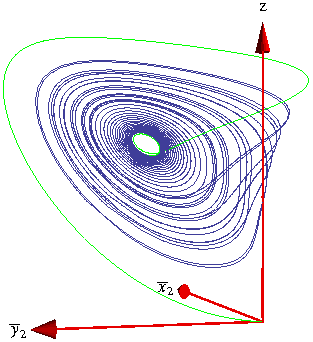
\includegraphics[width=0.35\textwidth,clip=true]{../figs/CLEinvXYZ}
~~~~(\textit{b})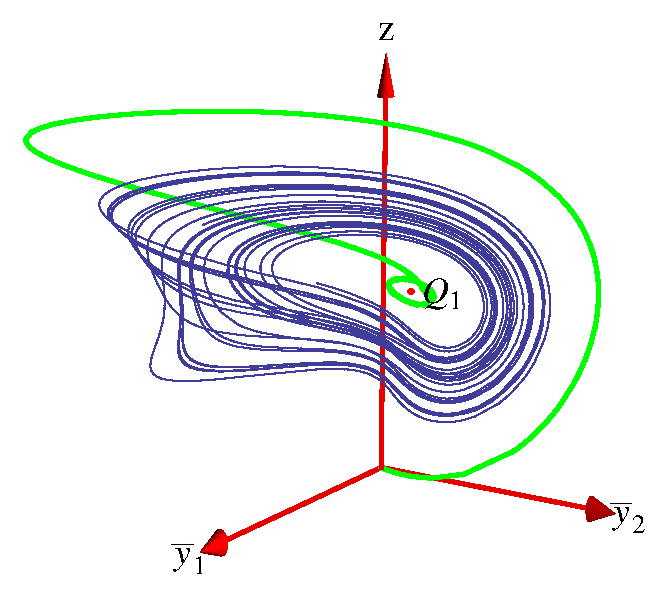
\includegraphics[width=0.35\textwidth,clip=true]{../figs/CLEinvYYZ}
\end{center}
\caption{
\Statesp\ portraits of \cLf\  in \reducedsp,
projected on invariant coordinates \refeq{eq:invLaser2}.
    }
\label{fig:CLEinv}
\end{figure}
%%%%%%%%%%%%%%%%%%%%%%%%%%%%%%%%%%%%%%%%%%%%%%%%%%%%%%%%%%%%%%%%

%%%%%%%%%%%%%%%%%%%%%%%%%%%%%%%%%%%%%%%%%%%%%%%%%%%%%%%%%%%%%%%%%%
\begin{figure}[ht]
\begin{center}
%   (\textit{a})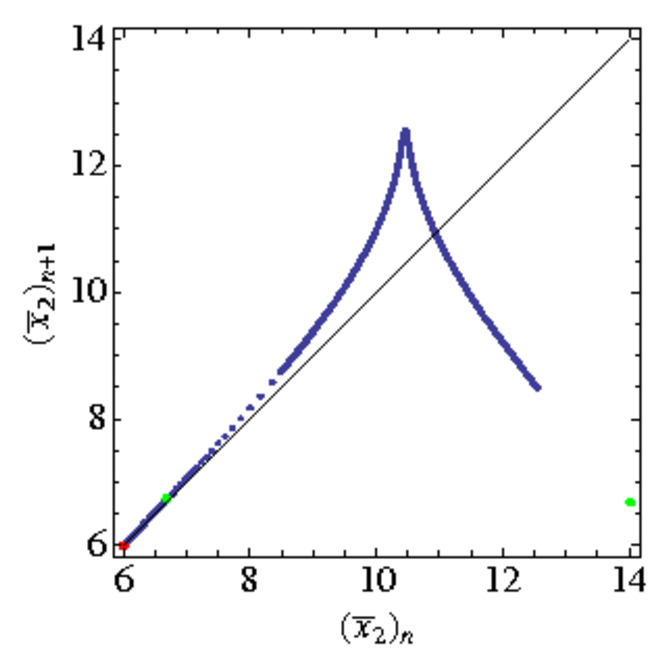
\includegraphics[width=0.35\textwidth,clip=true]{../figs/CLEinvRMx2}
%  ~~~~(\textit{b})
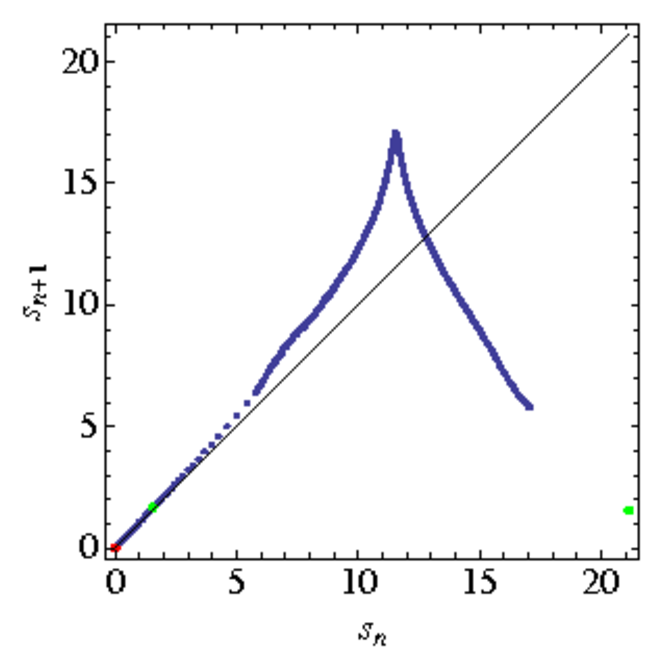
\includegraphics[width=0.35\textwidth,clip=true]{../figs/CLEinvRM}
\end{center}
\caption[Return map for Complex Lorenz flow]{
Return map to the \Poincare\ surface of section
$\overline{x}_2=\overline{y}_2$ for \cLe\ with $e=1/10$,
$\ImrCLor=0$, projecting on invariants given in
\refeq{eq:invLaser2}. The return map coordinate is the
Euclidean length along the \Poincare\ section of the unstable
manifold of $E_1$.
    }
\label{fig:CLEinvRM}
\end{figure}
%%%%%%%%%%%%%%%%%%%%%%%%%%%%%%%%%%%%%%%%%%%%%%%%%%%%%%%%%%%%%%%%

{\bf PC 2010-01-27:}
is the sign of the Lie algebra generator
\refeq{CLfLieGen}, group element standard?

{\bf ES 2010-01-28:}
    No. According
to Byron and Fuller, Mathematics of Classical and Quantum
Physics, which I find a very reliable and carefully written
book, what I use right now is the convention most physicists
use for \emph{active} transformations. This I've also used
in thesis and I'd be happy to stick with this. With this choice
small angle, active rotations, are counterclockwise, so I've updated
our orientation condition as well.

{\bf PC 2010-01-28:} Thanks, let's make sure that we have the
right sign in discrete.tex, continuous.tex (once CLE.tex is
submitted). Never seen Byron and Fuller.


{\bf PC  2010-01-28:} in \reffig{fig:CLEpcSect}:\\
        * please, no both this figure and 'coincidentally'
          \reffig{fig:CLEmfReqb1}. \Mframes\ and \mslices\ are
          \emph{identical}, former is the integral version of the latter,
          so this is an embarrassing claim. The reduced flows are of course
          one and the same for the same choice of the slice point.
	  {\bf ES} With the integral
	  version we can ``pass'' through singularities, while with the differential
	  version they pose a real difficulty. So I want to let the reader know that
	  here we can obtain the same figure with both.
          \\
        * I think it is a bad idea too plot both $\{x_1,x_2,z\}$ and
          $\{y_1,y_2,z\}$ projections. They are too tightly coupled, and
          look very much the same. That is why in ChaosBook I plot
          $\{x_1,x_2,z\}$ and
          $\{x_1,y_2,z\}$ projections; the latter exhibits the sharp
          singular space discontinuity.
        * Mark $\ssp_{\REQB{}1}$ \\
        * Draw stable eigenvector of $\ssp_{\REQB{}1}$\\
        * State value of $\ssp_{\REQB{}1}$ somewhere
     {\bf ES:} Agreed. Draw stable eigenvector of $\ssp_{\REQB{}1}$? Not sure this would look
		  nice at this scale, I will instead indicate direction of motion along unstable
		manifold of \EQV{0} by arrow.

%%%%%%%%%%%%%%%%%%%%%%%%%%%%%%%%%%%%%%%%%%%%%%%%%%%%%%%%%%%%%%%%
%computed with vaggelis/testing/flows/CLEfinalTmp.nb
\begin{figure}[ht]
\begin{center}
  (\textit{a})%kept 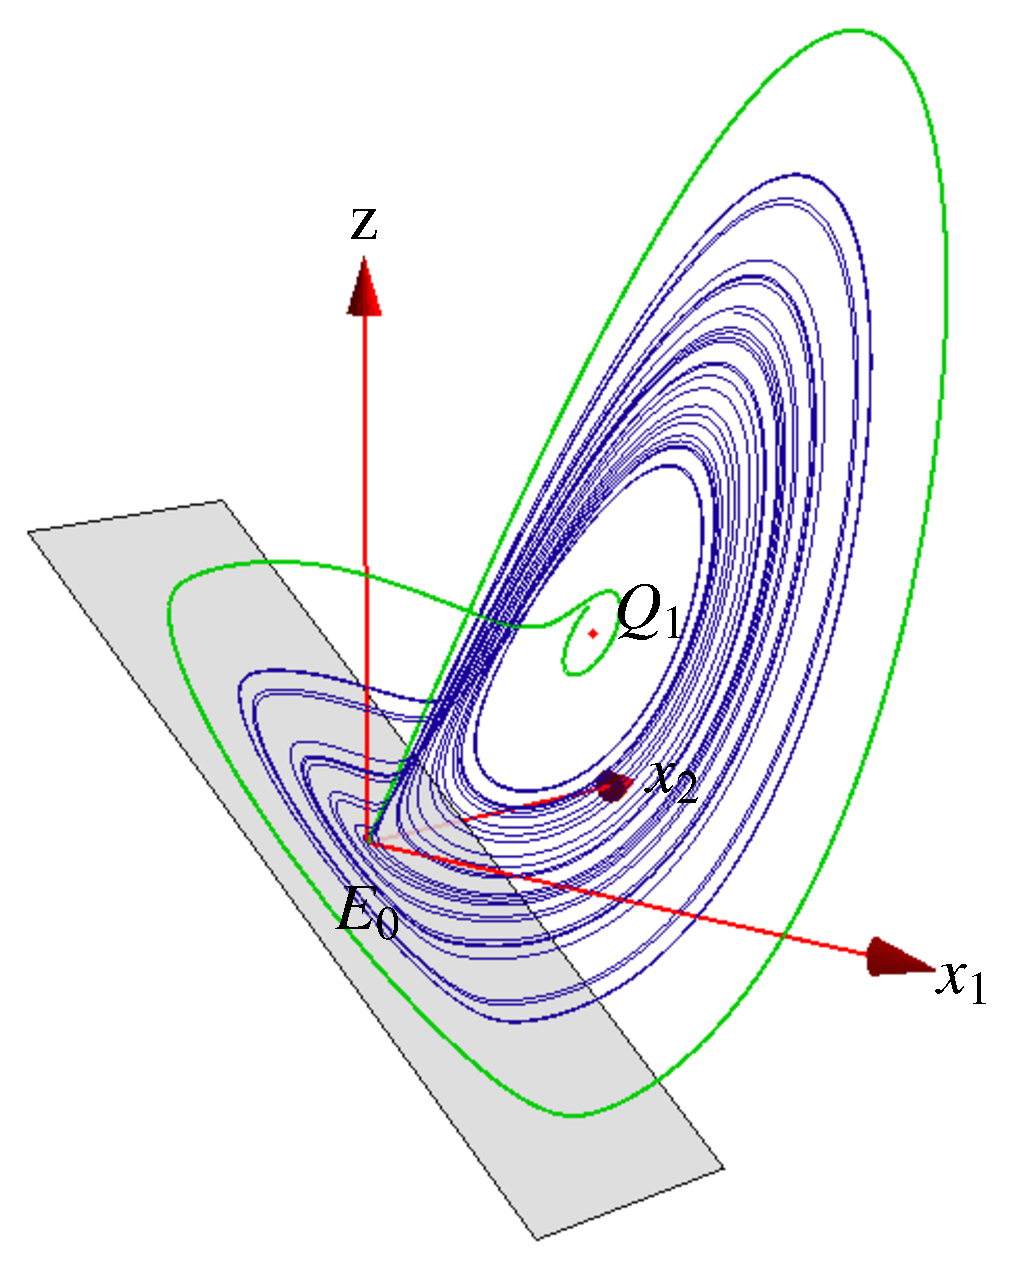
\includegraphics[width=0.35\textwidth,clip=true]{../figs/CLEmfReqb123}
~~~~(\textit{b})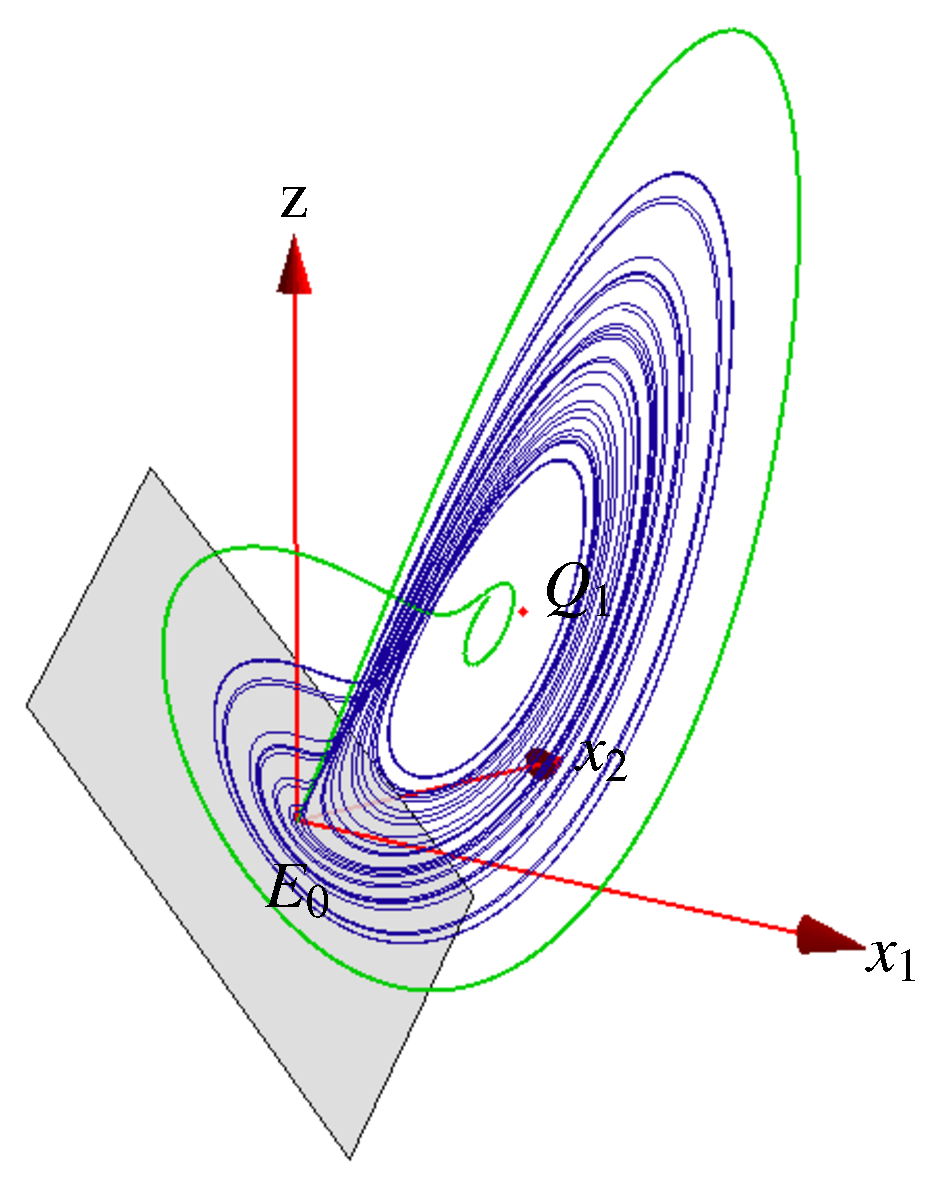
\includegraphics[width=0.35\textwidth,clip=true]{../figs/CLEmfAdHoc123}
\end{center}
\caption{
\Statesp\ portraits of \cLf\ in \reducedsp. We use a
moving frame map to a slice orthogonal to the group tangent
at  (a) $\slicep  = \ssp_{\REQB{1}}$, (b) $\slicep  =
\ssp_{\REQB{1}}+(0,-5,0,0,0)$. The gray plane indicates the \sset.
    }\label{fig:CLEmfssetOld}
\end{figure}
%%%%%%%%%%%%%%%%%%%%%%%%%%%%%%%%%%%%%%%%%%%%%%%%%%%%%%%%%%%%%%%%

%%%%%%%%%%%%%%%%%%%%%%%%%%%%%%%%%%%%%%%%%%%%%%%%%%%%%%%%%%%%%%%%
%computed with vaggelis/testing/flows/CLEfinalTmp.nb
\begin{figure}[ht]
\begin{center}
  (\textit{a})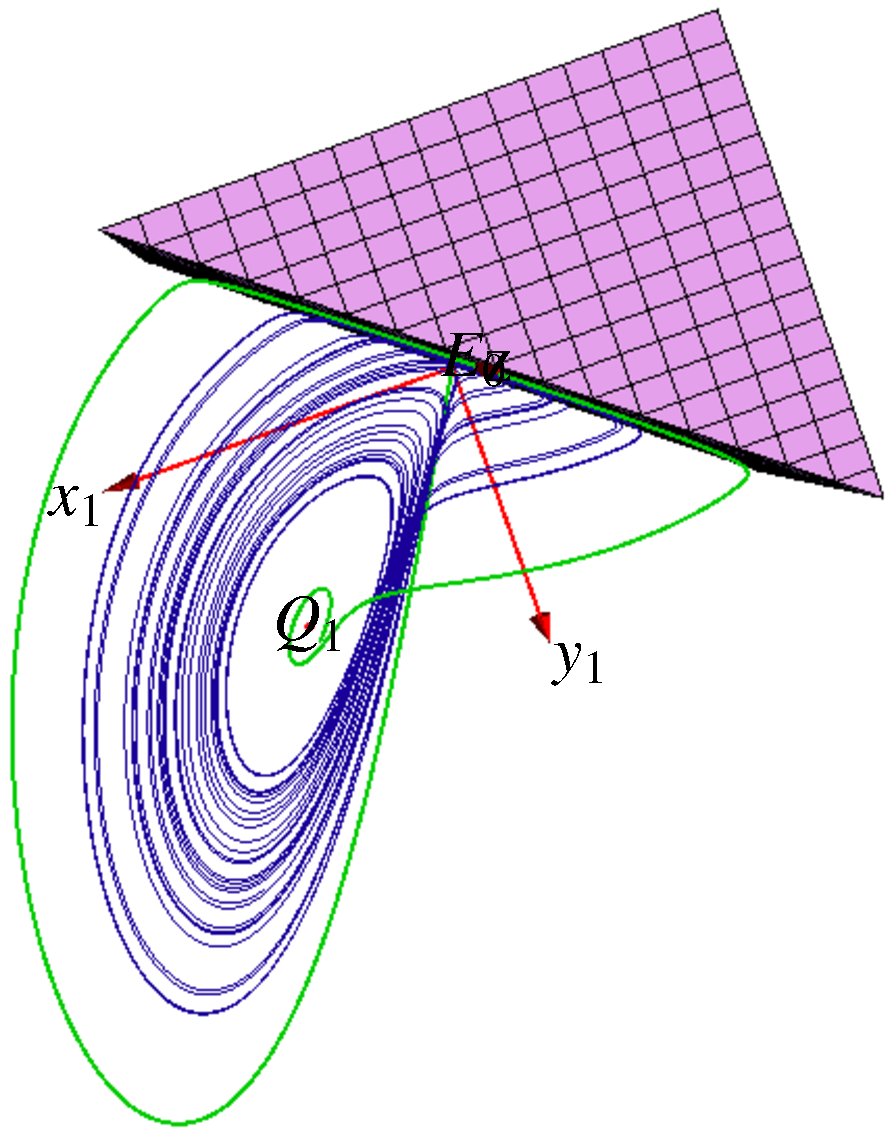
\includegraphics[width=0.35\textwidth,clip=true]{../figs/CLEmfReqb135}
~~~~(\textit{b})% kept 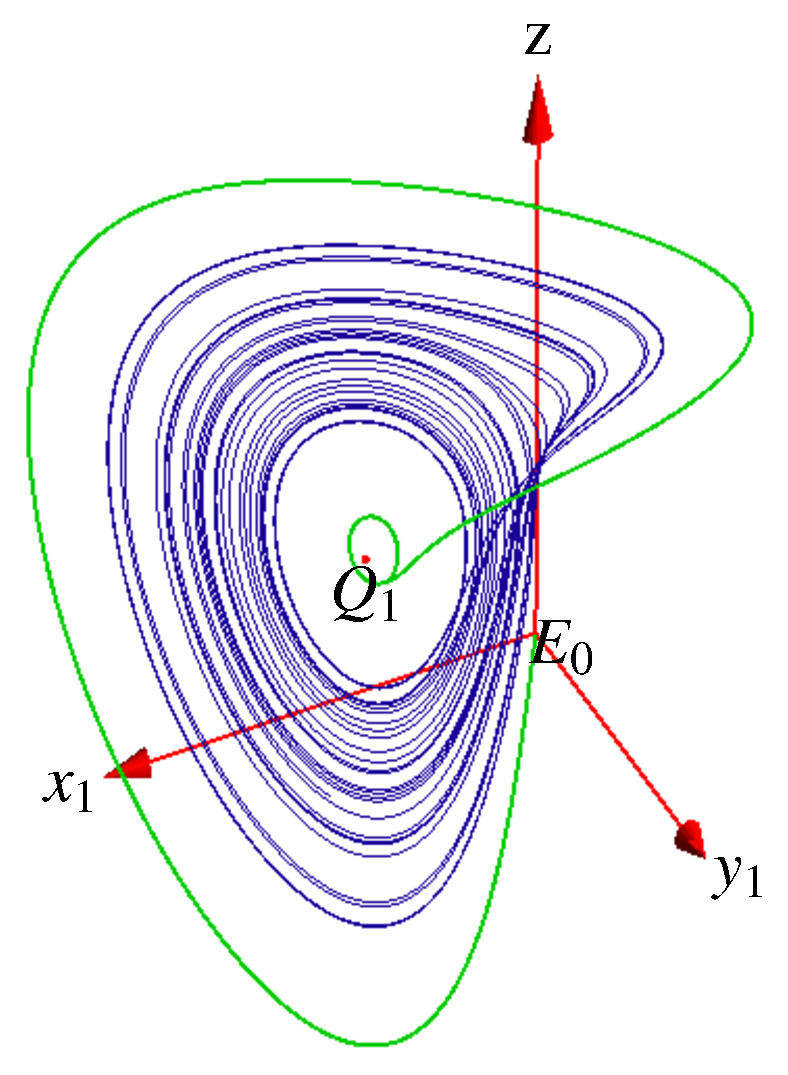
\includegraphics[width=0.35\textwidth,clip=true]{../figs/CLEmfAdHoc135}
\end{center}
\caption{
\Statesp\ portraits of \cLf\ in \reducedsp. We use a
moving frame map to a slice orthogonal to the group tangent
at  (a) $\slicep  = \ssp_{\REQB{1}}$, (b) $\slicep  =
\ssp_{\REQB{1}}+(0,-5,0,0,0)$. The shaded area indicates the \sset.
    }
\label{fig:CLEmfAdHoc}
\end{figure}
%%%%%%%%%%%%%%%%%%%%%%%%%%%%%%%%%%%%%%%%%%%%%%%%%%%%%%%%%%%%%%%%

%%%%%%%%%%%%%%%%%%%%%%%%%%%%%%%%%%%%%%%%%%%%%%%%%%%%%%%%%%%%%%%%
\begin{figure}[ht]
\begin{center}
  (\textit{a})% kept this 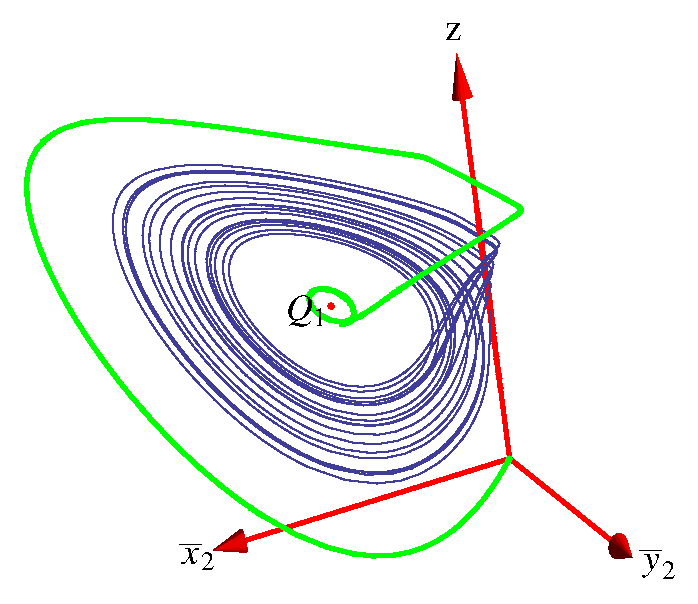
\includegraphics[width=0.35\textwidth,clip=true]{../figs/CLEmfXYZ}
 ~~~~(\textit{b})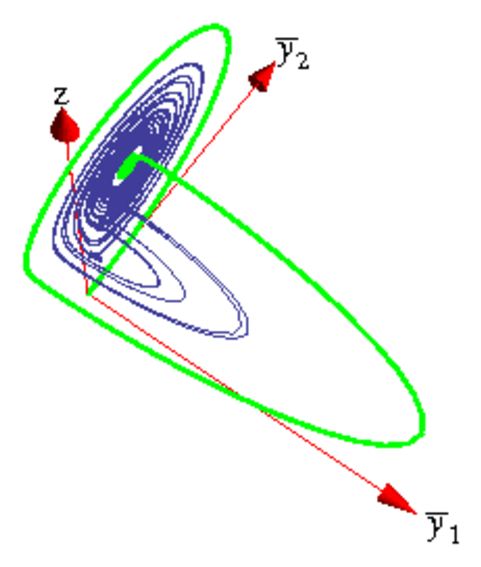
\includegraphics[width=0.35\textwidth,clip=true]{../figs/CLEmfYYZ}
\end{center}
\caption{
(a) \Statesp\ portrait of \cLf\ in \reducedsp,
projected on invariant coordinates  \refeq{eq:invLaser},
(b) The return map for the \Poincare\ surface of section $\sspRed_2=\sspRed_4$
for \cLe\ projected on invariant coordinates \refeq{eq:invLaser}.
The return map coordinate is the Euclidean length along the
\Poincare\ section of the unstable manifold of $\REQB{1}$.
    }
\label{fig:CLEmfOld}
\end{figure}
%%%%%%%%%%%%%%%%%%%%%%%%%%%%%%%%%%%%%%%%%%%%%%%%%%%%%%%%%%%%%%%%

%
%%%%%%%%%%%%%%%%%%%%%%%%%%%%%%%%%%%%%%%%%%%%%%%%%%%%%%%%%%%%%%%%
%computed with vaggelis/testing/flows/CLEfinalTmp.nb
\begin{figure}[ht]
\begin{center}
  (\textit{a})\includegraphics[width=0.35\textwidth,clip=true]{../figs/CLEperpReqb1}
~~~~(\textit{b}) % kept this: \includegraphics[width=0.35\textwidth,clip=true]{../figs/CLEperpReqb}
\end{center}
\caption{
\Statesp\ portraits of \cLf\ in \reducedsp. We use a
moving frame map to a slice orthogonal to the group tangent
at  $\slicep  = \ssp_{\REQB{1}}$.
    }
\label{fig:CLEmfReqb1}
\end{figure}
%%%%%%%%%%%%%%%%%%%%%%%%%%%%%%%%%%%%%%%%%%%%%%%%%%%%%%%%%%%%%%%%
%


% %%%%%%%%%%%%%%%%%%%%%%%%%%%%%%%%%%%%%%%%%%%%%%%%%%%%%%%%%%%%%%%%%%
% % computed in vaggelis/testing/flows/CLEfinalTmp.nb
% \begin{figure}[ht]
% \begin{center}
%  (\textit{a})\includegraphics[width=0.43\textwidth,clip=true]{CLEperpReqb1}
% ~(\textit{b}) \includegraphics[width=0.43\textwidth,clip=true]{CLEperpReqb}
% \end{center}
% \caption{
% \Statesp\ portraits of \cLf\  in \reducedsp\
% obtained by {\Mframes}, \slice\ fixed by a point on the
% \reqv\ group orbit, $\slicep  = \ssp_{\REQB{1}}$.
% (a) $\{x_1,x_2,z\}$ projection,
% (b) $\{y_1,y_2,z\}$ projection.
% }
% \label{fig:CLEpcSect}
% \end{figure}
% %%%%%%%%%%%%%%%%%%%%%%%%%%%%%%%%%%%%%%%%%%%%%%%%%%%%%%%%%%%%%%%%
%

% \PublicPrivate{}{
% % %%%%%%%%%%%%%%%%%%%%%%%%%%%%%%%%%%%%%%%%%%%%%%%%%%
% % % computed by PCunrot.nb
% % \SFIG{PCunrot1}
% % {}{
% % {\Mframes}, continuous time version, for the
% % polar coordinates motivated $x^{*}=(0,1,0,0)$,
% % $x_1=0,\;x_2>0$, \slice. The \cLf\ strange attractor of
% % \reffig{fig:CLE} exhibits a discontinuity at
% % $x_2=0$ in the \reducedsp:
% % $\{x_2,y_2,z\}$ projection.
% % }
% % {fig:PCunrot1}
% % %%%%%%%%%%%%%%%%%%%%%%%%%%%%%%%%%%%%%%%%%%%%%%%%%%
%
% Indeed, the method does encounter singularities in
% subsets of \statesp.
% For example, the \reducedsp\ equations \refeq{PCsectSin1}
% for the polar coordinates inspired \slice\
% $x^{*}=(0,1,0,0)$, $x_1=0,\;x_2>0$,
% %this is illustrated by \reffig{fig:PCunrot}.
% %$(\rho_1,\theta_1)$ are polar coordinates, $\rho_1 =
% %\sqrt{\ssp_1^{ 2} + \ssp_2^{2}}$, see \refeq{eq:CartToPol},
% are given by
% \beq
% \dot{\ssp} = \vel - \frac{\vel_1}{\ssp_2} \Lg \cdot \ssp
% \,.
% \ee{EqMotionMovFrame}
% A typical trajectory is shown in \reffig{fig:PCunrot}.
%    \PC{this is not \reffig{fig:PCunrot} - copy correct fig
%        from wilczak/blog
%        }
% }

%\renewcommand{\Group}{\ensuremath{\Gamma}}    % Siminos Lie group

{\bf PC 2010-01-29:} replaced these two by their sum:
\beq
\left(
\begin{array}{c}
\dot{\theta}_1\\
\dot{\theta}_2
\end{array}
\right)
=
\left(
\begin{array}{c}
-\sigma\frac{r_2}{r_1}\sin\theta  \\
 e + (\rho_1-z)\frac{r_1}{r_2}\sin\theta
\end{array}
\right)
\,.
\label{eq:PolarCLeAnglesOld}
\eeq

{\bf PC 2010-01-29 replaced by ChaosBook.org version:}

\beq
\begin{split}
\dot{\overline{x}}_1 &= 0\,\\
\dot{\overline{x}}_2 &=-\sigma  \left(\overline{x}_2-\overline{y}_2 \right)\,,\\
\dot{\overline{y}}_1 &=-\overline{y}_1- \left(e+\sigma\frac{\overline{y}_1}{\overline{x}_2} \right)\overline{y}_2\,,\\
\dot{\overline{y}}_2 &=(\RerCLor -z)\overline{x}_2+\left(e+\frac{\sigma  \overline{y}_1}{\overline{x}_2}
\right) \overline{y}_1-\overline{y}_2\,,\\
\dot{z} &=\overline{x}_2 \overline{y}_2-b z\,.
\end{split}
\eeq

{\bf PC 2010-01-29 dropped:}
    Looks like one should also read \refref{Abraham95}; they
    report on various return maps.

    CLEip1 was plotted by the devil, it is cool 2MB.

    {\bf PC} I think this is wrong, safer to drop it:
``In the \cLe\ example no
trajectories enter the $x_1=x_2=0$ subspace, but this is a
fortuitous event'' so I am dropping it. Without any loss of
information. {\bf ES} Do you think that generic trajectories do enter $x_1=x_2=0$
or that it is not a fortuitous event?

{\bf ES dropped text from stability appendix:}

Using the {\mframes} to map dynamics on a slice $\pSRed$ as
in refsect~{sec:mf} or restricting integration on the slice
as in refsect~{sec:MovFrameODE}, the reduced \statesp\ is
identified (at least locally) with the {\slice} ${\pSRed}$.
This provides a means of calculating stability of \reqva\ in
reduced \statesp. Proof that such a notion of stability of
\reqva\ is meaningful is given, for instance, in
\refref{Krupa90}.  To simplify notation we only treat
the one-dimensional group case and drop all group parameter
related indices, writing $\Lg_{ij}$ instead of
$(\Lg_1)_{ij}$, \etc.

{\bf ES to Predrag:}
 I couldn't find Chossat and Lauterbach book
    here. If you have it would it be easy to have a look at their
    expression for stability of \reqva? Is this claim correct? I
    remember that my motivation to derive it was that their
    expression is too implicit to use in practice, while Krupa's
    is totally abstract. But maybe I was missing something.
    {\bf PC:} no time for me to go to the library now
    and check this...

{\bf PC} the problem is that this formula is based on
    the \emph{method of connections} of Rowley
    \etal\rf{rowley_reduction_2003} which we cannot use
    because its additional \emph{geometric phase}. They prove
    a theorem
    - as well as probably Beyn - that it is OK for \reqva.

{\bf ES:} Yes, this is why we only use it for stability of \reqva.
	      I will have to try rpo stability using projection we use
	      for integration on the slice, but it is too late for this paper.
	      I had the well known problem back then, I did not understand
	      derivation of Rowley and Marsden.

In \ref{s:StabReq} we derive an expression for the stability
of \reqva\ (traveling waves) in \reducedsp\
that can be applied without an explicit
calculation of the reduced system.
    \PC{unless you clean up \ref{s:StabReq} now, it will have to
        be omitted.}

\section{\label{s:StabReq} Stability of \reqva}

{\bf PC 2010-01-27} this appendix stabReqva.tex from the thesis
        does not seem ready for the prime time.
        If we refer to it as in the above 'Public' version you
        will have to update your thesis.

%     \input stabReqva


\section{To fix}
% former siminos/CLE/05fixMe.tex

{\bf PC 2010-01-26} template says:
\begin{verbatim}
Use \appendix* if there only one appendix.
\end{verbatim}
but I do not see how to do it.
ES: Neither do I.

defsCLE.tex  2010-01-26 contains this:
\begin{verbatim}
\renewcommand\Poincare{Poincar\'e}
  % ES: It is {Poincar\'e } in ChaosBook, is this on purpose?
  % PC it's the same symbol, no?
  % ES: There is a trailing space in contrast to most macros.
  % No major issue, I'm just used to add an extra \ after macros
  % and with this it looks like too much white space.
\end{verbatim}

ES: Physica D seems to require corresponding author to be
designated by $\backslash$corref, but I cannot get it to work.
